\subsection{Heine--Borel and Euclidean Compactness}

\begin{theorem} \label{thm:nested-closed-intervals-intersect} \hlt{Nested Closed Intervals Intersect}\\
If $I_1\supseteq I_2\supseteq I_3\supseteq\cdots$ is a sequence of closed intervals in $\R$, then $\bigcap_{n=1}^{\infty}I_n\neq\emptyset$.
\begin{proof}
Let $I_n=[a_n,b_n]$. The set $\{a_n:n\in\N\}$ is nonempty and bounded above by each $b_m$.\\
Let $x=\sup\{a_n:n\in\N\}$. Then $a_m\leq x\leq b_m$ for every $m$, so $x\in I_m$ for all $m$.\\
\hlt{Structural Commentary}: Completeness traps a common point.\\
\hlt{Key Insight}: The least upper bound of the left endpoints lies in every interval.
\end{proof}
\end{theorem}

\begin{figure}[H]
  \centering
  \begin{tikzpicture}[
  scale=0.88,
  every node/.style={font=\small},
  axis/.style={gray!70, line width=0.55pt},
  interval/.style={blue!70!black, line width=0.85pt},
  tick/.style={gray!70, line width=0.55pt},
  supmark/.style={circle, fill=orange!80!black, inner sep=1.55pt}
]
  \draw[axis] (-4.5,0) -- (4.5,0);

  \coordinate (aone) at (-3.8,0);
  \coordinate (atwo) at (-2.8,0);
  \coordinate (athree) at (-1.8,0);
  \coordinate (an) at (-0.8,0);
  \coordinate (xstar) at (0.2,0);
  \coordinate (bn) at (1.2,0);
  \coordinate (bthree) at (2.2,0);
  \coordinate (btwo) at (3.2,0);
  \coordinate (bone) at (4.2,0);

  \draw[interval] ($(aone)+(0,0.45)$) -- ($(bone)+(0,0.45)$);
  \draw[interval] ($(atwo)+(0,0.85)$) -- ($(btwo)+(0,0.85)$);
  \draw[interval] ($(athree)+(0,1.25)$) -- ($(bthree)+(0,1.25)$);
  \draw[interval] ($(an)+(0,1.65)$) -- ($(bn)+(0,1.65)$);

  \foreach \pt/\lab in {aone/a_1,atwo/a_2,athree/a_3,an/a_n,bn/b_n,bthree/b_3,btwo/b_2,bone/b_1} {
    \draw[tick] (\pt) ++(0,-0.12) -- ++(0,0.24);
    \node[below] at ($(\pt)+(0,-0.12)$) {$\lab$};
  }

  \node[supmark] at (xstar) {};
  \draw[orange!80!black, line width=0.55pt] (xstar) ++(0,-0.22) -- ++(0,2.17);
  \node[above] at ($(xstar)+(0,1.95)$) {$x=\sup\{a_n:n\in\N\}$};

  \node[left] at ($(aone)+(0,0.45)$) {$I_1$};
  \node[left] at ($(atwo)+(0,0.85)$) {$I_2$};
  \node[left] at ($(athree)+(0,1.25)$) {$I_3$};
  \node[left] at ($(an)+(0,1.65)$) {$I_n$};
\end{tikzpicture}

  \caption{For nested closed intervals $[a_n,b_n]$, supremum of left endpoints lies between every $a_n$ and $b_n$.}
  \label{fig:nested-closed-intervals-lub}
\end{figure}

\begin{theorem} \label{thm:nested-k-cells-intersect} \hlt{Nested $k$-Cells Intersect}\\
If $I_1\supseteq I_2\supseteq I_3\supseteq\cdots$ is a sequence of $k$-cells in $\R^k$, then $\bigcap_{n=1}^{\infty}I_n\neq\emptyset$.
\begin{proof}
Let $I_n=\{\mathbf{x}\in\R^k:a_{n,j}\leq x_j\leq b_{n,j},\ 1\leq j\leq k\}$. For each coordinate $j$, the intervals $[a_{n,j},b_{n,j}]$ are nested, so Theorem \ref{thm:nested-closed-intervals-intersect} gives a point $x_j^*$ lying in all of them. Then $\mathbf{x}^*=(x_1^*,\ldots,x_k^*)$ lies in every $I_n$.\\
\hlt{Structural Commentary}: A nested cell problem reduces coordinatewise to nested intervals.\\
\hlt{Key Insight}: Choose one persistent coordinate at a time.
\end{proof}
\end{theorem}

\begin{figure}[H]
  \centering
  \begin{tikzpicture}[
  every node/.style={font=\small},
  axis/.style={->, gray!70, line width=0.5pt},
  cell/.style={draw=blue!65!black, fill=blue!12, line width=0.75pt},
  edge/.style={blue!65!black, line width=0.75pt},
  hidden/.style={blue!65!black, dashed, dash pattern=on 2pt off 2pt, line width=0.55pt},
  tick/.style={gray!70, line width=0.5pt}
]
  \begin{scope}
    \draw[axis] (-0.2,0) -- (2.6,0);
    \draw[cell] (0.55,-0.08) rectangle (2.0,0.08);
    \draw[tick] (0.55,-0.18) -- (0.55,0.18);
    \draw[tick] (2.0,-0.18) -- (2.0,0.18);
    \node[below] at (0.55,-0.18) {$a_1$};
    \node[below] at (2.0,-0.18) {$b_1$};
    \node[above] at (1.25,0.35) {$1$-cell};
  \end{scope}

  \begin{scope}[xshift=3.3cm]
    \draw[axis] (-0.2,0) -- (2.8,0);
    \draw[axis] (0,-0.2) -- (0,2.2);
    \draw[cell] (0.7,0.55) rectangle (2.25,1.75);
    \draw[tick] (0.7,-0.12) -- (0.7,0.12);
    \draw[tick] (2.25,-0.12) -- (2.25,0.12);
    \draw[tick] (-0.12,0.55) -- (0.12,0.55);
    \draw[tick] (-0.12,1.75) -- (0.12,1.75);
    \node[below] at (0.7,-0.12) {$a_1$};
    \node[below] at (2.25,-0.12) {$b_1$};
    \node[left] at (-0.12,0.55) {$a_2$};
    \node[left] at (-0.12,1.75) {$b_2$};
    \node[above] at (1.4,2.15) {$2$-cell};
  \end{scope}

  \begin{scope}[xshift=7.0cm]
    \draw[axis] (-0.2,0) -- (2.9,0);
    \draw[axis] (0,-0.2) -- (0,2.25);
    \draw[axis] (-0.1,-0.1) -- (1.1,1.1);
    \coordinate (A) at (0.7,0.55);
    \coordinate (B) at (1.95,0.55);
    \coordinate (C) at (1.95,1.5);
    \coordinate (D) at (0.7,1.5);
    \coordinate (s) at (0.55,0.45);
    \fill[blue!12] (A) -- (B) -- (C) -- (D) -- cycle;
    \fill[blue!8] ($(A)+(s)$) -- ($(B)+(s)$) -- ($(C)+(s)$) -- ($(D)+(s)$) -- cycle;
    \draw[edge] (A) -- (B) -- (C) -- (D) -- cycle;
    \draw[edge] ($(A)+(s)$) -- ($(B)+(s)$) -- ($(C)+(s)$) -- ($(D)+(s)$) -- cycle;
    \draw[edge] (B) -- ($(B)+(s)$);
    \draw[edge] (C) -- ($(C)+(s)$);
    \draw[edge] (D) -- ($(D)+(s)$);
    \draw[hidden] (A) -- ($(A)+(s)$);
    \node[below] at (0.7,-0.08) {$a_1$};
    \node[below] at (2.5,-0.08) {$b_1$};
    \node[left] at (-0.08,0.55) {$a_2$};
    \node[left] at (-0.08,1.5) {$b_2$};
    \node[right] at ($(B)+(s)+(0.05,0)$) {$b_3$};
    \node[above] at (1.45,2.15) {$3$-cell};
  \end{scope}
\end{tikzpicture}

  \caption{A $1$-cell is a closed interval, a $2$-cell is a coordinate rectangle, and a $3$-cell is a coordinate box.}
  \label{fig:k-cell-low-dimensional-examples}
\end{figure}

\begin{theorem} \label{thm:k-cells-compact} \hlt{$k$-Cells Are Compact}\\
Every $k$-cell in $\R^k$ is compact.
\begin{proof}
Let $I=\{\mathbf{x}:a_j\leq x_j\leq b_j,\ 1\leq j\leq k\}$ and set $\delta\defeq\left(\sum
\limits_{j=1}^{k}(b_j-a_j)^2\right)^{1/2}$. Suppose an open cover $\{G_\alpha\}$ of $I$ has no finite subcover. Bisect each coordinate interval. Among the resulting $2^k$ subcells, at least one cannot be finitely covered by the $G_\alpha$; call it $I_1$. Continue inductively, obtaining nested cells $I\supseteq I_1\supseteq I_2\supseteq\cdots$ such that no $I_n$ is finitely covered and every two points of $I_n$ are within $2^{-n}\delta$ of each other.\\
By Theorem \ref{thm:nested-k-cells-intersect}, choose $\mathbf{x}^*\in\bigcap_n I_n$. Since $\{G_\alpha\}$ covers $I$, some $G_\alpha$ contains $\mathbf{x}^*$. Because $G_\alpha$ is open, $B_r(\mathbf{x}^*)\subseteq G_\alpha$ for some $r>0$. By the Archimedean property in Theorem \ref{thm:archimedean-and-rational-density}, choose $n$ with $n>\delta/r$; since $2^n\geq n$, we have $2^{-n}\delta<r$. Then $I_n\subseteq G_\alpha$, contradicting the construction of $I_n$.\\
\hlt{Structural Commentary}: Repeated bisection traps a point in cells whose diameters shrink to zero.\\
\hlt{Key Insight}: An open set around the trapped point eventually contains the whole small cell.
\end{proof}
\end{theorem}

\begin{figure}[H]
  \centering
  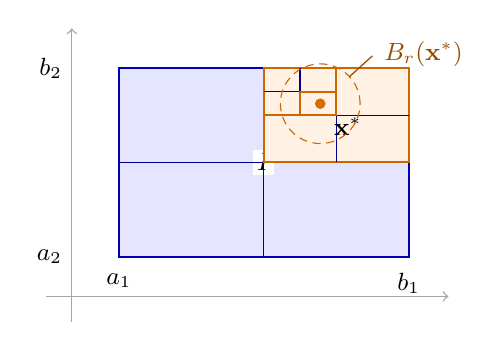
\begin{tikzpicture}[
  scale=0.92,
  every node/.style={font=\small},
  axis/.style={->, gray!70, line width=0.5pt},
  cell/.style={draw=blue!70!black, fill=blue!10, line width=0.75pt},
  subcell/.style={draw=blue!55!black, line width=0.45pt},
  focus/.style={draw=orange!80!black, fill=orange!10, line width=0.75pt},
  point/.style={circle, fill=orange!85!black, inner sep=1.35pt}
]
  \draw[axis] (-0.35,0) -- (5.2,0);
  \draw[axis] (0,-0.35) -- (0,3.7);

  \coordinate (A) at (0.65,0.55);
  \coordinate (B) at (4.65,0.55);
  \coordinate (C) at (4.65,3.15);
  \coordinate (D) at (0.65,3.15);

  \draw[cell] (A) rectangle (C);
  \node[fill=white, inner sep=1.5pt] at (2.65,1.85) {$I$};

  \draw[subcell] (2.65,0.55) -- (2.65,3.15);
  \draw[subcell] (0.65,1.85) -- (4.65,1.85);

  \draw[focus] (2.65,1.85) rectangle (4.65,3.15);
  \draw[subcell] (3.65,1.85) -- (3.65,3.15);
  \draw[subcell] (2.65,2.5) -- (4.65,2.5);

  \draw[focus] (2.65,2.5) rectangle (3.65,3.15);
  \draw[subcell] (3.15,2.5) -- (3.15,3.15);
  \draw[subcell] (2.65,2.825) -- (3.65,2.825);

  \draw[focus] (3.15,2.5) rectangle (3.65,2.825);
  \node[point,label=below right:$\mathbf{x}^\ast$] at (3.43,2.66) {};

  \node[below] at (0.65,0.45) {$a_1$};
  \node[below] at (4.65,0.45) {$b_1$};
  \node[left] at (0.0,0.55) {$a_2$};
  \node[left] at (0.0,3.15) {$b_2$};

  \draw[orange!80!black, dashed, dash pattern=on 3pt off 2pt] (3.43,2.66) circle (0.55);
  \draw[orange!60!black, line width=0.45pt] (3.83,3.03) -- (4.15,3.32);
  \node[orange!60!black, anchor=west] at (4.18,3.34) {$B_r(\mathbf{x}^\ast)$};
\end{tikzpicture}

  \caption{Repeated bisection traps a point.}
  \label{fig:k-cell-bisection-compactness}
\end{figure}

\begin{lemma} \label{lem:bounded-rk-set-contained-in-k-cell} \hlt{Bounded Euclidean Sets Fit in $k$-Cells}\\
Every bounded subset $E\subseteq\R^k$ is contained in some $k$-cell.
\begin{proof}
If $E=\emptyset$, any $k$-cell contains $E$. Suppose $E\neq\emptyset$. By Definition \ref{def:bounded-and-perfect-metric-sets}, choose $\mathbf{q}=(q_1,\ldots,q_k)\in\R^k$ and $M>0$ such that $\norm{\mathbf{p}-\mathbf{q}}_2<M$ for all $\mathbf{p}\in E$. Let $I\defeq\{\mathbf{x}=(x_1,\ldots,x_k):q_j-M\leq x_j\leq q_j+M,\ 1\leq j\leq k\}$.\\
For $\mathbf{p}=(p_1,\ldots,p_k)\in E$, $\abs{p_j-q_j}\leq\norm{\mathbf{p}-\mathbf{q}}_2<M$ for each $j$, so $\mathbf{p}\in I$.\\
Thus $E\subseteq I$, and $I$ is a $k$-cell by Definition \ref{def:euclidean-intervals-cells-balls-convex}.\\
\hlt{Structural Commentary}: A Euclidean ball centered at $\mathbf{q}$ sits inside the coordinate box with side half-length $M$.\\
\hlt{Key Insight}: Boundedness supplies one radius; coordinates turn it into interval bounds.
\end{proof}
\end{lemma}

\begin{theorem} \label{thm:heine-borel-rk} \hlt{Heine--Borel in $\R^k$}\\
For $E\subseteq\R^k$, any one of the following three properties implies the other two:
\begin{enumerate}[label=(\roman*)]
\setlength{\itemsep}{0pt}
\item $E$ is closed and bounded;
\item $E$ is compact;
\item every infinite subset of $E$ has a limit point in $E$.
\end{enumerate}
\begin{proof}
\begin{enumerate}[label=(\roman*)]
\setlength{\itemsep}{0pt}
\item[$(i)$]$\Rightarrow(ii)$: Since $E$ is bounded, Lemma \ref{lem:bounded-rk-set-contained-in-k-cell} gives $E\subseteq I$ for some $k$-cell $I$. By Theorem \ref{thm:k-cells-compact}, $I$ is compact; since $E$ is closed, Theorem \ref{thm:closed-subsets-of-compact-sets-compact} gives that $E$ is compact.
\item[$(ii)$]$\Rightarrow(iii)$: This is Theorem \ref{thm:infinite-subset-of-compact-has-limit-point}.
\item[$(iii)$]$\Rightarrow(i)$: If $E$ is unbounded, choose $\mathbf{x}_n\in E$ with $\norm{\mathbf{x}_n}_2>n$ and set $S\defeq\{\mathbf{x}_n:n\in\N\}$. If $\mathbf{x}_n\in B_R(\mathbf{y})$, then $n<\norm{\mathbf{y}}_2+R$; hence $S$ has no limit point, contradicting (iii). Thus $E$ is bounded. If $E$ is not closed, choose $\mathbf{x}_0\in E^{\operatorname{acc}}\setminus E$ and $\mathbf{x}_n\in E$ with $0<\norm{\mathbf{x}_n-\mathbf{x}_0}_2<1/n$. Then $S\defeq\{\mathbf{x}_n:n\in\N\}$ is infinite and $S^{\operatorname{acc}}\subseteq\{\mathbf{x}_0\}\subseteq E^c$, contradicting (iii). Thus $E$ is closed.
\end{enumerate}
\hlt{Structural Commentary}: In $\R^k$, the three tests coincide.\\
\hlt{Key Insight}: Heine--Borel is the bridge between open-cover compactness and Euclidean bounded geometry.
\end{proof}
\end{theorem}

\begin{corollary} \label{cor:heine-borel-real-line-sequential-form} \hlt{Heine--Borel on the Real Line}\\
For $E\subseteq\R$, the following are equivalent:
\begin{enumerate}[label=(\roman*)]
\setlength{\itemsep}{0pt}
\item $E$ is closed and bounded;
\item $E$ is compact;
\item every sequence in $E$ has a subsequence converging to a point of $E$.
\end{enumerate}
\begin{proof}
\begin{enumerate}[label=(\roman*).]
\setlength{\itemsep}{0pt}
\item[$(i)$]$\Rightarrow (ii)$ Since $E\subseteq\R=\R^1$ is closed and bounded, Theorem \ref{thm:heine-borel-rk} with $k=1$ implies $E$ is compact.
\item[$(ii)$]$\Rightarrow (iii)$ Compactness and Theorem \ref{thm:compact-complete-totally-bounded} give convergent subsequence; compactness keeps limit in $E$.
\item[$(iii)$]$\Rightarrow (i)$ Let $F\subseteq E$ be infinite. Choose distinct $x_n\in F$ using Principle \ref{princ:axiom-of-choice-analysis}. By (iii), some $x_{n_j}\to x\in E$. Since the $x_n$ are distinct, $x$ is a limit point of $F$ in the sense of Definition \ref{def:metric-topology-core-definitions}. Hence every infinite subset of $E$ has a limit point in $E$, so Theorem \ref{thm:heine-borel-rk} gives that $E$ is closed and bounded.
\end{enumerate}
\hlt{Structural Commentary}: Real-line compactness equals closed-bounded sequential compactness.\\
\hlt{Key Insight}: Closed bounded sets keep sequences from escaping.
\end{proof}
\end{corollary}

\begin{corollary} \label{cor:nested-closed-bounded-real-sets-intersect} \hlt{Nested Closed Bounded Real Sets Intersect}\\
Let $(F_n)_{n\in\N}$ be nonempty closed subsets of $\R$ with $F_{n+1}\subseteq F_n$ for all $n$. If $F_1$ is bounded, then $\bigcap_{n=1}^{\infty}F_n\neq\emptyset$.
\begin{proof}
By Corollary \ref{cor:heine-borel-real-line-sequential-form}, $F_1$ is compact. For each $n$, $F_n$ is closed in $\R$, $F_n\subseteq F_1$, and $F_n\ne\emptyset$; hence $F_n$ is a nonempty compact subset of $F_1$ by Theorem \ref{thm:closed-subsets-of-compact-sets-compact}. Since $F_{n+1}\subseteq F_n$, Corollary \ref{cor:nested-nonempty-compact-intersection} gives $\bigcap_{n=1}^{\infty}F_n\neq\emptyset$.\\
\hlt{Structural Commentary}: Compact nested sets have the finite-intersection property.\\
\hlt{Key Insight}: Heine--Borel upgrades the real-line nested set theorem to compactness.
\end{proof}
\end{corollary}

\begin{theorem} \label{thm:weierstrass-limit-point-rk} \hlt{Weierstrass Limit-Point Theorem}\\
Every bounded infinite subset of $\R^k$ has a limit point in $\R^k$.
\begin{proof}
By Lemma \ref{lem:bounded-rk-set-contained-in-k-cell}, a bounded set $E$ lies in some $k$-cell $I$. By Theorem \ref{thm:k-cells-compact}, $I$ is compact.\\
Since $E$ is an infinite subset of $I$, Theorem \ref{thm:infinite-subset-of-compact-has-limit-point} gives a limit point of $E$ in $I\subseteq\R^k$.\\
\hlt{Structural Commentary}: Boundedness places the set inside a compact cell.\\
\hlt{Key Insight}: Compact cells force bounded infinite sets to accumulate.
\end{proof}
\end{theorem}
